\chapter{Platforma od strony użytkowej}
\label{chapter:interfaces}

Stroną startową platformy jest ekran logowania użytkownika.
Uwierzytelnienie użytkownika odbywa się z użyciem serwisu GitHub (opis techniczny procesu znajduje się w podrodziale \label{authorization}).
Po poprawnym zalogowaniu użytkownik, w zależności od swoich uprawnień zostaje przekierowany do odpowiedniego widoku.
W przypadku prowadzącego będzie to ekran wyboru zarządzania projektami lub podglądu postępów studentów.
Użytkownik będący studentem zostanie przekierowany do widoku dostępnych dla niego projektów.

Opis ekranu logowania znajduje się w podrozdziale \ref{fe_login}.
W kolejnym rozdziale zostały omówione interfejsy dostępne dla prowadzącego.
Ostatni podrozdział zawiera opis widoku studenta.

\section{Panel logowania}
\label{fe_login}

Panel logowania umożliwia uwierzytelnienie z użyciem serwisu GitHub.
Po kliknięciu przycisku ”Zaloguj” użytkownik jest przekierowywany na stronę logowania GitHub.
W serwisie można zalogować się poprzez podanie maila bądź nazwy użytkownika i hasła.
Należy też wyraziź zgodę na przetwarzanie danych przez platformę.
Po poprawnym zalogowaniu użytkownik zostaje przekierowany spowrotem na stronę platformy.
Po przetworzeniu danych uwierzytelniających przez platformę użytkownikowi wyświetalny jest kolejny ekran, zależny od jego uprawnień.
Na rysunkach od \ref{fig:log_in_butoon} do \ref{fig:wait_for_login} zostały przedstawione kolejne ekrany związane z procesem logowania.

\begin{figure}[h]
    \centering
    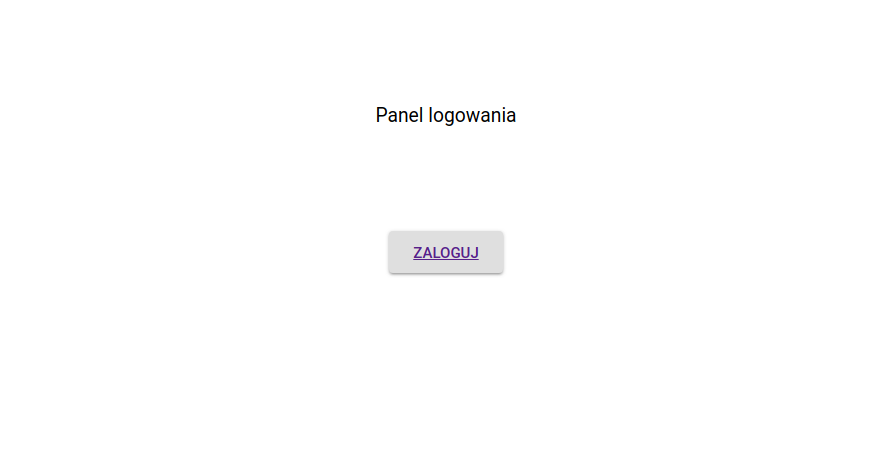
\includegraphics[width = 8cm]{chapter04/log_in_button.png}
    \caption{Ekran logowania w ramach platformy (źródło własne).}
    \label{fig:log_in_butoon}
\end{figure}

\begin{figure}[h]
    \centering
    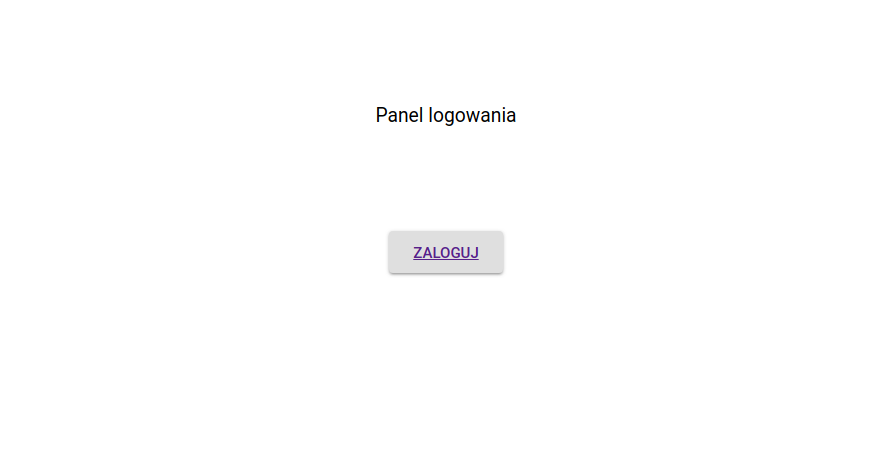
\includegraphics[width = 8cm]{chapter04/log_in_button.png}
    \caption{Ekran logowania do serwisu GitHub (źródło własne).}
    \label{fig:log_in_butoon}
\end{figure}

\begin{figure}[H]
    \centering
    
\includegraphics[width = 8cm]{chapter04/wait_for_login.png}
    \caption{Ekran oczekiwania na zalogowanie w ramach platformy (źródło własne).}
    \label{fig:wait_for_login}
\end{figure}

\section{Interfejs prowadzącego}

Jeśli zalogowany użytkownik posiad uprawnienia prowadzącego (administratora) po poprawnym zalogowaniu wyświetlany jest mu ekran wyboru zarządzania projektami lub podglądu postępów grup.
Ekran wyboru akcji został zamieszczony na rysunku \ref{fig:lecturer_actions}.

\begin{figure}[h]
    \centering
    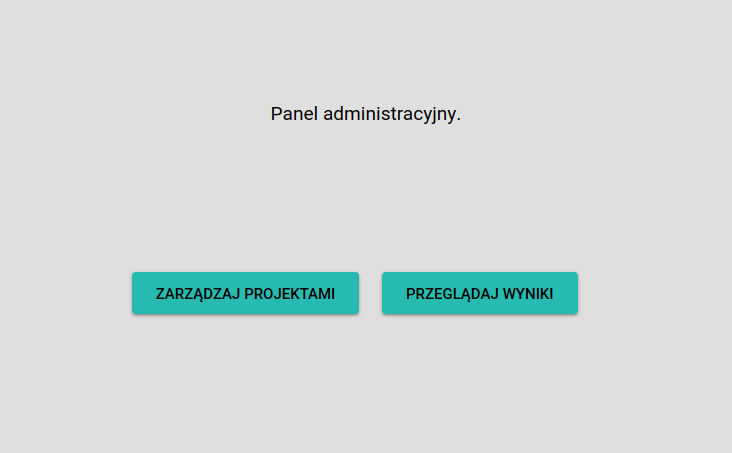
\includegraphics[width = 8cm]{chapter04/lecturer_actions.png}
    \caption{Ekran oczekiwania na zalogowanie w ramach platformy (źródło własne).}
    \label{fig:lecturer_actions}
\end{figure}

Omówienie widoku zarządzania projektami znajduje się w podrozdziale \ref{lecturer-management}.
Opis interfejsu podglądu postępów studentów został zamieszczony w sekcji \ref{lecturer_preview}.

\subsection{Zarządzanie projektami}
\label{lecturer-management}

W ramach zarządzania udostępnione jest tworzenie i edytowanie projektów, w tym wyznaczanie etapów i integracji oraz dodawanie do nich przypadków testowych.
Definiowanie projektu sprowadza się do:
\begin {itemize}
    \item Utworzenia nowego projektu.
    \item Dodania etapów wraz z przypadkami testowymi.
    \item Utworzenia procesów integracji wraz z przypadkami testowymi.
    \item Dodania grup projektowych.
\end {itemize}

Dla wszystkich parametrów będących plikami interfejs umożliwia dodanie ich poprzez wskazanie, w oknie dialogowym, ścieżki na dysku użytkownika, pod którą znajduje się plik.

Na rysunku \ref{fig:lecturer_projects_list} został przedstawiony podstawowy widok zarządzania projektami zawierający listę dostępnych projektów.
Na tym ekranie prowadzący może przejść do wybranego projektu, usunąć go lub utworzyć nowy projekt.
Lista dostępnych projektów jest posortowana alfabetycznie po ich nazwie.

\begin{figure}[h]
    \centering
    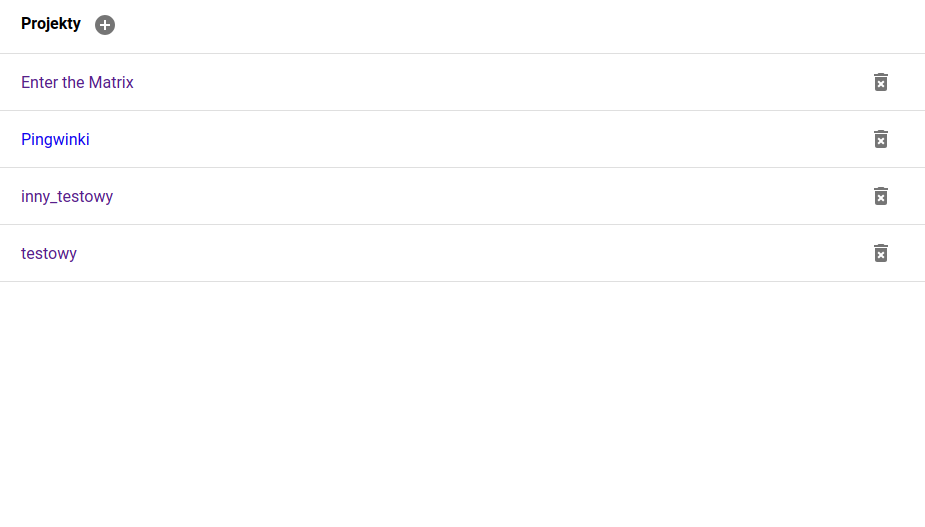
\includegraphics[width = 8cm]{chapter04/lecturer_projects_list.png}
    \caption{Interfejs prowadzącego, zarządzanie projektami - lista projektów (źródło własne).}
    \label{fig:lecturer_projects_list}
\end{figure}

Widok projektu oraz panele etapów, grup i integracji zostały omówione w ramach kolejnych sekcji.

\subsubsection{Widok projektu}

Projekt definiowany jest przez następujące dane:
\begin {itemize}
    \item Nazwę projektu, która jest jednoznaczna z nazwą katalogu na dysku, w którym przechowywane będą pliki z danymi dotyczącymi projektu.
    Nazwa jest parametrem będącym ciągiem znaków (String).
    \item Plik z opisem projektu o dowolnym formacie.
    \item Plik Dockerfile definiujący środowisko uruchomieniowe programów.
    \item Listę etapów.
    \item Listę grup.
    \item Listę integracji.
\end {itemize}

Na rysunku \ref{fig:lecturer_project_board} przedstawiono podstawowy widok projektu.

\begin{figure}[h]
    \centering
    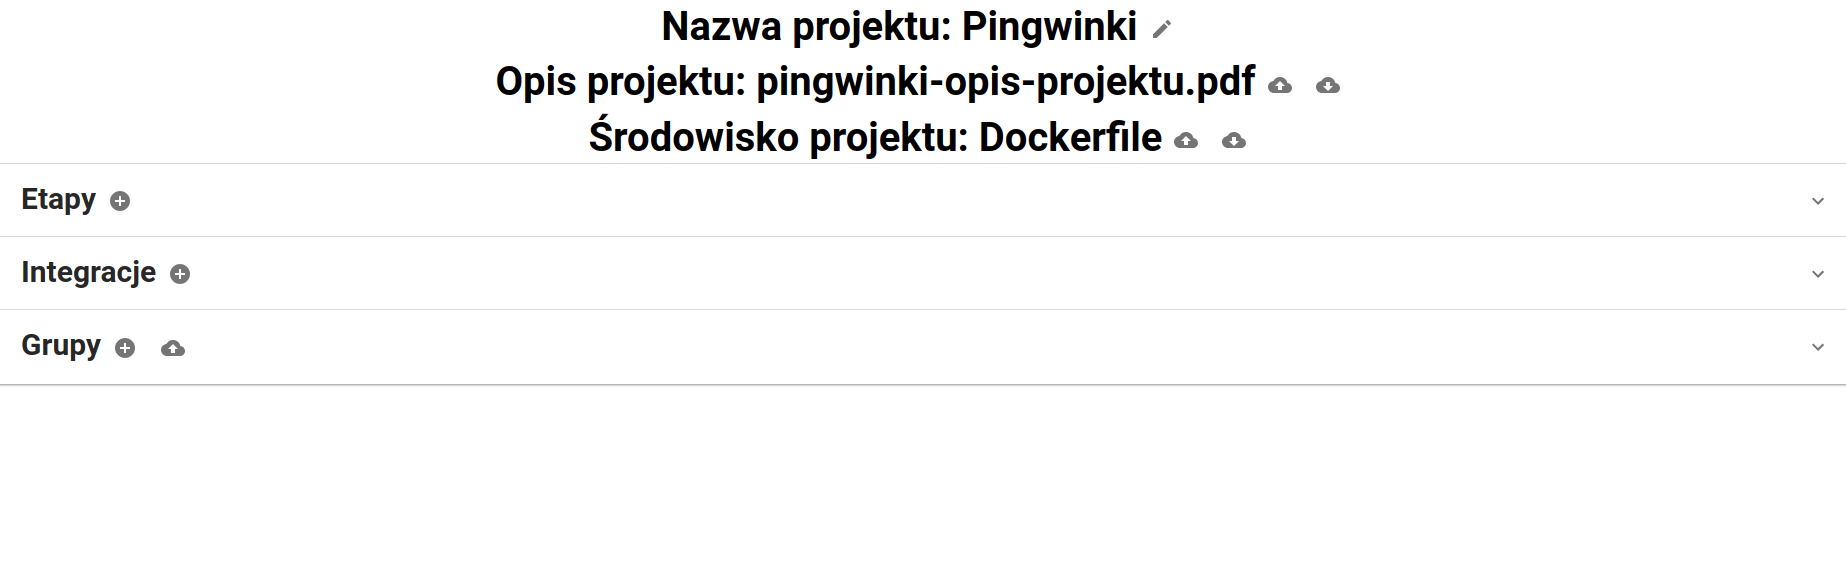
\includegraphics[width = 13cm]{chapter04/lecturer_project_board.png}
    \caption{Interfejs prowadzącego, zarządzanie projektami - widok projektu (źródło własne).}
    \label{fig:lecturer_project_board}
\end{figure}

\subsubsection{Panel etapów}

Etap definiowany jest przez następujące dane:
\begin {itemize}
    \item Nazwę etapu, która jest jednoznaczna z nazwą katalogu na dysku, w którym przechowywane będą pliki z danymi dotyczącymi etapu.
    Nazwa jest parametrem będącym ciągiem znaków (String).
    \item Plik z opisem etapu o dowolnym formacie.
    \item Metadane dotyczące etapu, takie jak:
    \begin {itemize}
        \item Data rozpoczęcia etapu.
        Data rozpoczęcia jest rozumiana jako data, od której studenci mają możliwość rozpoczęcia prac nad etapem (dostęp do opisu etapu, możliwość zaimportowania i uruchomienia swoich programów),
        \item Data zakończenia etapu.
        Data zakończenia jest rozumiana jako data, do której studenci mają możliwość zaimportowania i uruchomienia swoich programów.
        Po przekroczeniu tej daty zmian programów i ponownych uruchomień może dokonywać tylko prowadzący.
        \item Komentarz do etapu.
        Jest on dodatkową informacją widoczną tylko dla prowadzącego.
    \end{itemize}
\end {itemize}

Etapy, które nie mają zdefiniowanej daty rozpoczęcia nie są widoczne dla studentów.
Interfejs umożliwia wskazanie daty poprzez wybór jej w oknie dialogowym z kalendarzem.

Na rysunku \ref{fig:lecturer_stages} został przedstawiony przykładowy panel etapów.
Komentarz do etapu wyświetlany jest po najechaniu na ikonę reprezentującą dodatkowe informacje.

\begin{figure}[h]
    \centering
    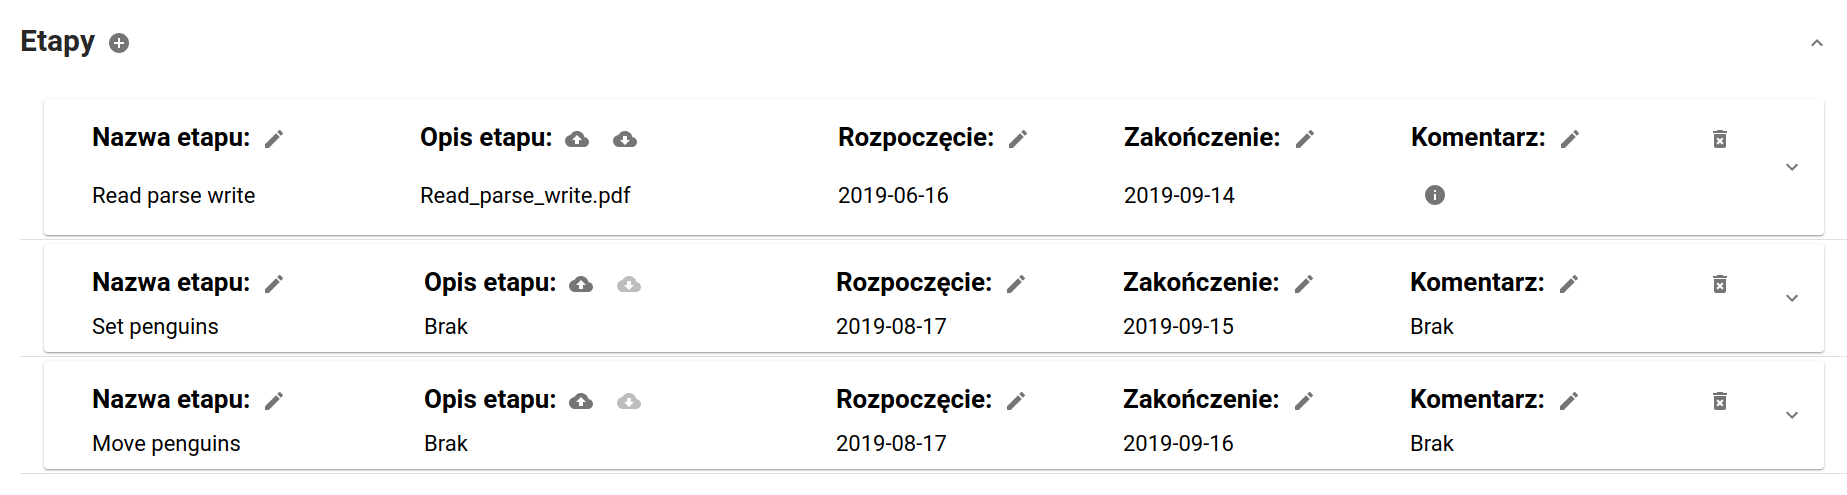
\includegraphics[width = 15cm]{chapter04/lecturer_stages.png}
    \caption{Interfejs prowadzącego, zarządzanie projektami - panel etapów (źródło własne).}
    \label{fig:lecturer_stages}
\end{figure}

W ramach panelu można dodawać, edytować oraz usuwać etapy.


Dla każdego z etapów można rozwinąć panel zawierający listę zdefiniowanych testów.
Opis uruchamianie i testowania programów studentów w ramach etapów został zamieszczony w rodziale \ref{chapter:platform-technical}.
Pojedynczy przypadek testowy jest definiowany przez następujące dane:
\begin {itemize}
    \item Nazwę przypadku testowego, która jest jednoznaczna z nazwą katalogu na dysku, w którym przechowywane będą pliki z danymi dotyczącymi tego przypadku.
    Nazwa jest parametrem będącym ciągiem znaków(String).
    \item Parametry uruchomienia programu, podawane jako plik.
    \item Plik z danymi wejściowymi dla zadanego przypadku o dowolnym, najczęściej tekstowym, formacie.
    Plik wejściowy jest używany jako dana wejściowa dla danego przypadku testowego.
    \item oczekiwany plik wyjściowy dla zadanego przypadku o dowolnym, najczęściej tekstowym, formacie.
    Oczekiwany plik wyjściowy jest używany do porównania wyniku otrzymanego w rezultacie działania programów studentów i na jego podstawie oceniana jest poprawność programów.
\end {itemize}

Rysunek \ref{fig:lecturer_stages_tests} przedstawia przykładowy panel zawierający testy dla etapu.

\begin{figure}[h]
    \centering
    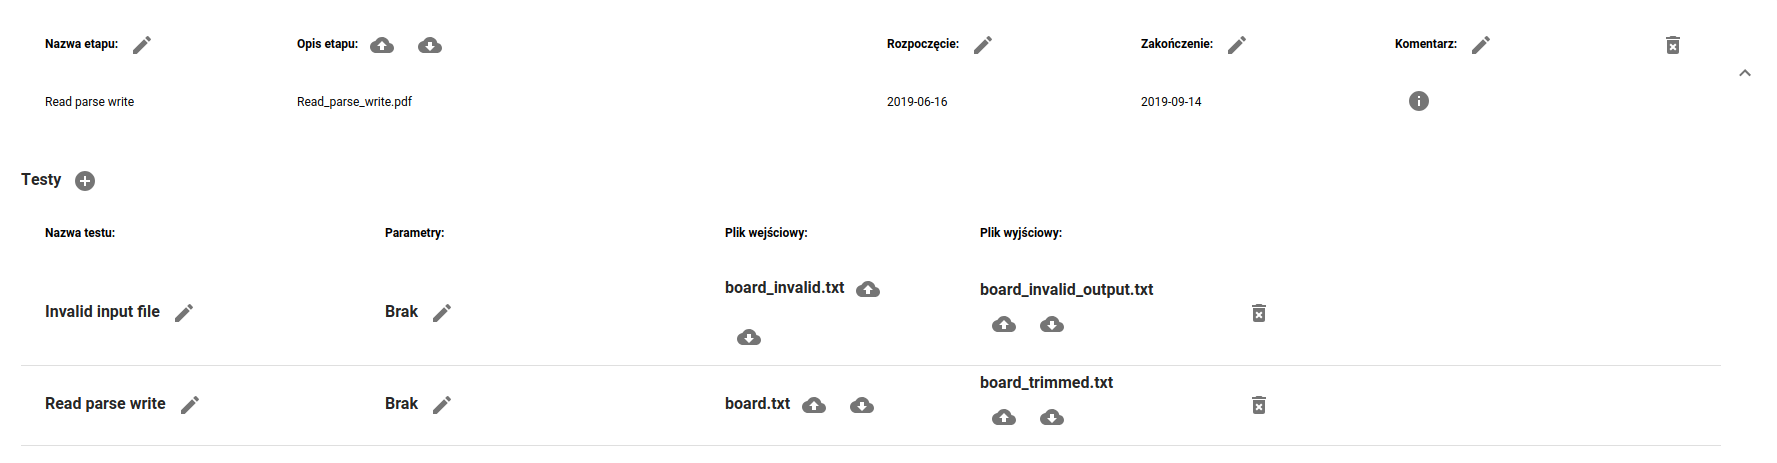
\includegraphics[width = 15cm]{chapter04/lecturer_stages_tests.png}
    \caption{Interfejs prowadzącego, zarządzanie projektami - panel testów dla etapu (źródło własne).}
    \label{fig:lecturer_stages_tests}
\end{figure}

W ramach każdego z paneli można dodawać, edytować oraz usuwać przypadki testowe.

\subsubsection{Panel integracji}

Proces integracji jest definiowany przez następujące dane:
\begin {itemize}
    \item Nazwę procesu, która jest jednoznaczna z nazwą katalogu na dysku, w którym przechowywane będą pliki z danymi dotyczącymi tego procesu.
    Nazwa jest parametrem będącym ciągiem znaków (String).
    \item Priorytetyzowaną listę etapów, które zostaną wykonane kolejno w ramach procesu integracji.
    \item Komentarz do etapu.
    Jest on dodatkową informacją widoczną tylko dla prowadzącego.
\end {itemize}

Na rysunku \ref{fig:lecturer_integrations} został przedstawiony przykładowy panel integracji.

\begin{figure}[h]
    \centering
    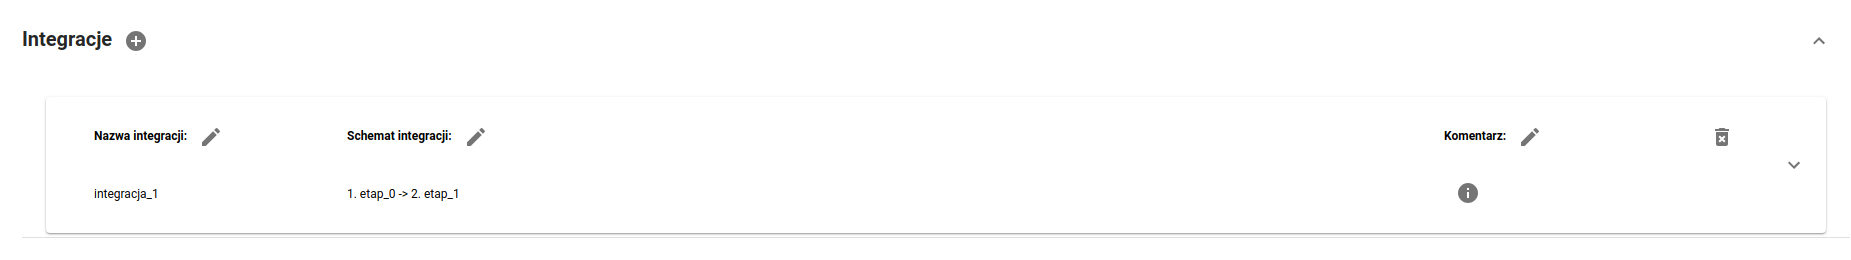
\includegraphics[width = 15cm]{chapter04/lecturer_integrations.png}
    \caption{Interfejs prowadzącego, zarządzanie projektami - panel integracji (źródło własne).}
    \label{fig:lecturer_integrations}
\end{figure}

Dla każdej z integracji można rozwinąć panel zawierający listę zdefiniowanych testów.
Opis uruchamianie i testowania programów studentów w ramach procesu integracji został zamieszczony w rodziale \ref{chapter:platform-technical}.
Pojedynczy przypadek testowy jest definiowany przez następujące dane:
\begin {itemize}
    \item Nazwę przypadku testowego, która jest jednoznaczna z nazwą katalogu na dysku, w którym przechowywane będą pliki z danymi dotyczącymi tego przypadku.
    Nazwa jest parametrem będącym ciągiem znaków(String).
    \item Parametry uruchomienia programu, podawane jako pliki.
    Dla każdego z etapów integracji podawane są oddzielne parametry wykonania w ramach jednego testu.
    \item Plik z danymi wejściowymi dla zadanego przypadku o dowolnym, najczęściej tekstowym, formacie.
    Plik wejściowy jest używany jako dana wejściowa dla danego przypadku testowego i jest pojedynczy w ramach jednego testu.
    \item oczekiwany plik wyjściowy dla zadanego przypadku o dowolnym, najczęściej tekstowym, formacie.
    Oczekiwany plik wyjściowy jest używany do porównania wyniku otrzymanego w rezultacie działania programów studentów i na jego podstawie oceniana jest poprawność programów.
    Oczekiwany plik wyjściowy jest pojedynczy w ramach jednego testu.
\end {itemize}

\begin{figure}[h]
    \centering
    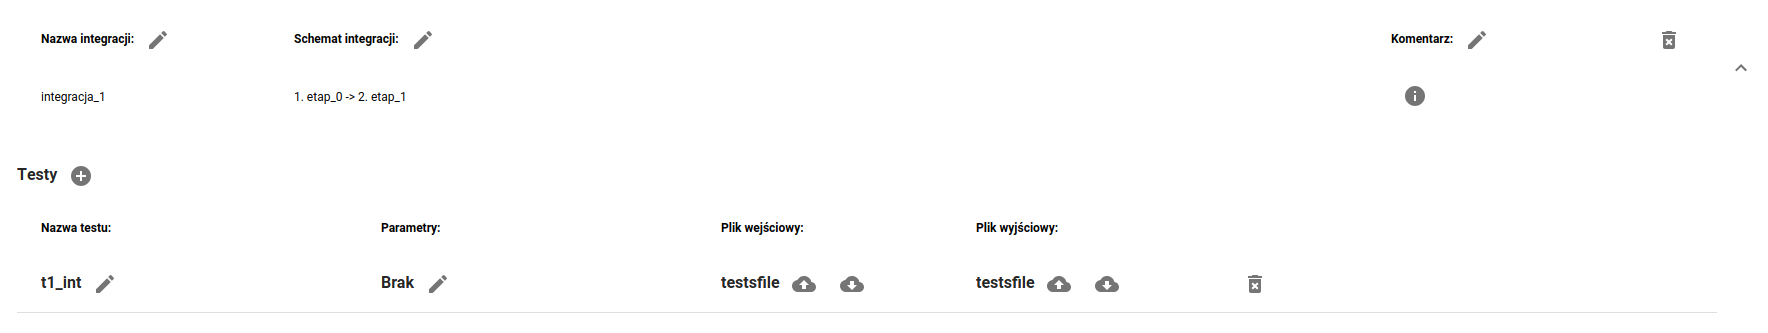
\includegraphics[width = 15cm]{chapter04/lecturer_integrations_tests.png}
    \caption{Interfejs prowadzącego, zarządzanie projektami - panel testów dla integracji (źródło własne).}
    \label{fig:lecturer_integrations_tests}
\end{figure}

W ramach każdego z paneli można dodawać, edytować oraz usuwać przypadki testowe.

\subsubsection{Panel grup}

W ramach panelu prowadzący ma możliwość utworzenia grup projektowych wraz z przypisaniem do nich studentów.
Na rysunku \ref{fig:lecturer_groups} zamieszczono widok rozwiniętego panelu grup.
Kolejny rysunek \ref{fig:lecturer_students_in_group} przedstawia rozwiniętą listę studentów przypisanych do danego zespołu

\begin{figure}[h]
    \centering
    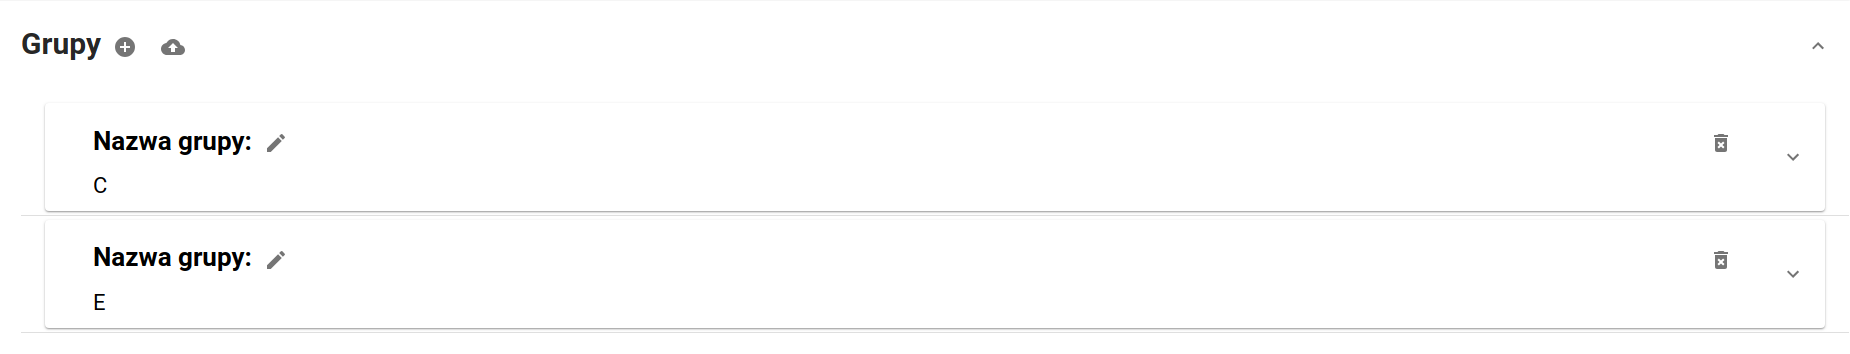
\includegraphics[width = 13cm]{chapter04/lecturer_groups.png}
    \caption{Interfejs prowadzącego, zarządzanie projektami - panel grup (źródło własne).}
    \label{fig:lecturer_groups}
\end{figure}

\begin{figure}[h]
    \centering
    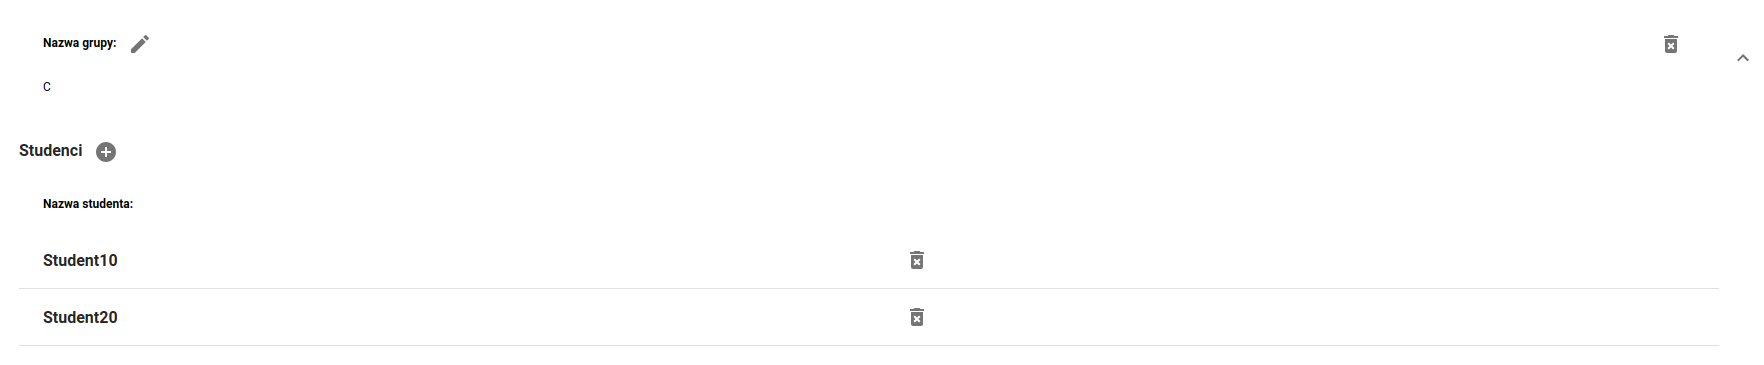
\includegraphics[width = 13cm]{chapter04/lecturer_students_in_group.png}
    \caption{Interfejs prowadzącego, zarządzanie projektami - panel grupy wraz z przypisanymi studentami (źródło własne).}
    \label{fig:lecturer_students_in_group}
\end{figure}

Utworzenie grup projektowych może zostać zrealizowane na dwa sposoby.
Pierwszy z nich to manualne utworzenie grup, definiowanych przez nazwę i dodanie kolejnych studentów w oknie dialogowym.
Aby dodać grupy manualnie należy użyć przycisku ”+” znajdującego się obok etykiety \textit{Grupy}.
Drugim sposobem załącznia grup jest wczytanie danych dotyczących z pliku w formacie JSON.
Przykład struktury akceptowalnego pliku został zamieszczony w podrozdziale \ref{adding_project_groups}.
W celu wczytania grup bezpośrednio z pliku należy użyć przycisku wgrywania danych znajdującego się obok etykiety \textit{Grupy}.

W ramach panelu umożliwiona jest edycja grup i studentów.

\subsection{Podgląd postępów studentów}
\label{lecturer_preview}

W ramach podglądu postępów studentów umożliwione jest:
\begin {itemize}
    \item Sprawdzenie statusu prac w ramach etapów i integracji dla każdej ze zdefiniowanych w ramach projektu grup.
    \item Uruchomienie programów.
    \item Edycja danych (programu, raportu, kodu) przez prowadzącego.
    \item Pobranie pliku zawierającego statystyki uruchomień w ramach integracji i etapów.
\end {itemize}

Prowadzący ma możliwość edycji danych studentów z uprawnieniami administratora.
Pozwalają one między innymi na edycję wprowadzonych przez studentów danych po upływie terminów realizacji poszczególnych etapów.
Są to uprawnienia, które nie powinny być nadużywane przez prowadzącego, jednak mogą okazać się użyteczne w wyjątkowych sytuacjach.

Na rysunku \ref{fig:lecturer_preview_projects_list} został przedstawiony podstawowy widok zarządzania projektami zawierający listę dostępnych projektów.
Poprzez ten ekran prowadzący może przejść do wybranego projektu.
Lista dostępnych projektów jest posortowana alfabetycznie po ich nazwie.

\begin{figure}[h]
    \centering
    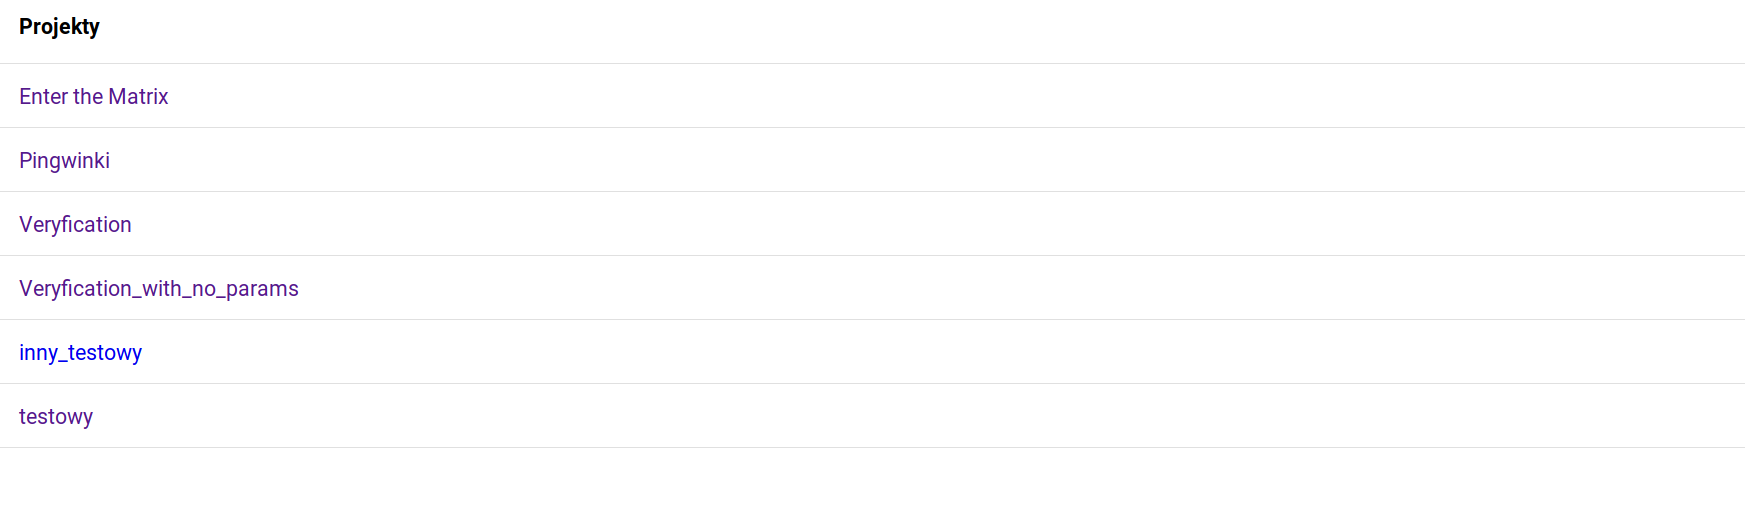
\includegraphics[width = 13cm]{chapter04/lecturer_preview_projects_list.png}
    \caption{Interfejs prowadzącego, podgląd postępów - lista projektów (źródło własne).}
    \label{fig:lecturer_preview_projects_list}
\end{figure}

Po przejściu do odpowiedniego projektu wyświetlany jest ekran z listą grup i studentów przypisanych do danego projektu.
Poprzez ten ekran prowadzący może przejść do rezultatów wybranego zespołu.
Lista grup jest posortowana alfabetycznie po nazwie.
Przykładowy ekran wyboru zespołu projektowego został zamieszczony na rysunku \ref{fig:lecturer_preview_groups}

\begin{figure}[h]
    \centering
    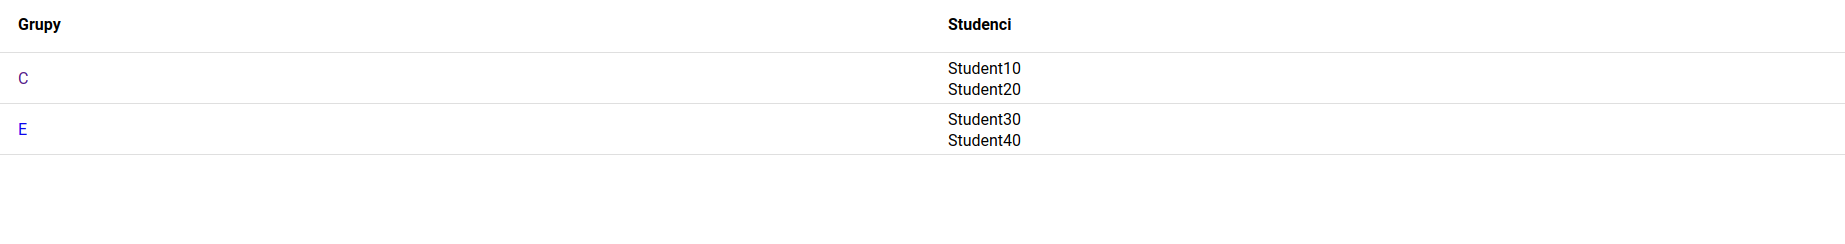
\includegraphics[width = 13cm]{chapter04/lecturer_preview_groups.png}
    \caption{Interfejs prowadzącego, podgląd postępów - lista grup (źródło własne).}
    \label{fig:lecturer_preview_groups}
\end{figure}



\subsubsection{Pogląd postępów w ramach etapu}

Na rysunku \ref{fig:lecturer-interface-view} został przedstawiony widok podglądu postępów studentów.
W ramach interfejsu prowadzący ma możliwość przeglądania postępów za równo poprzez wyszukanie po nazwie grupy, jak i po identyfikatorze poszczególnych studentów.

\begin{figure}[h]
    \centering
    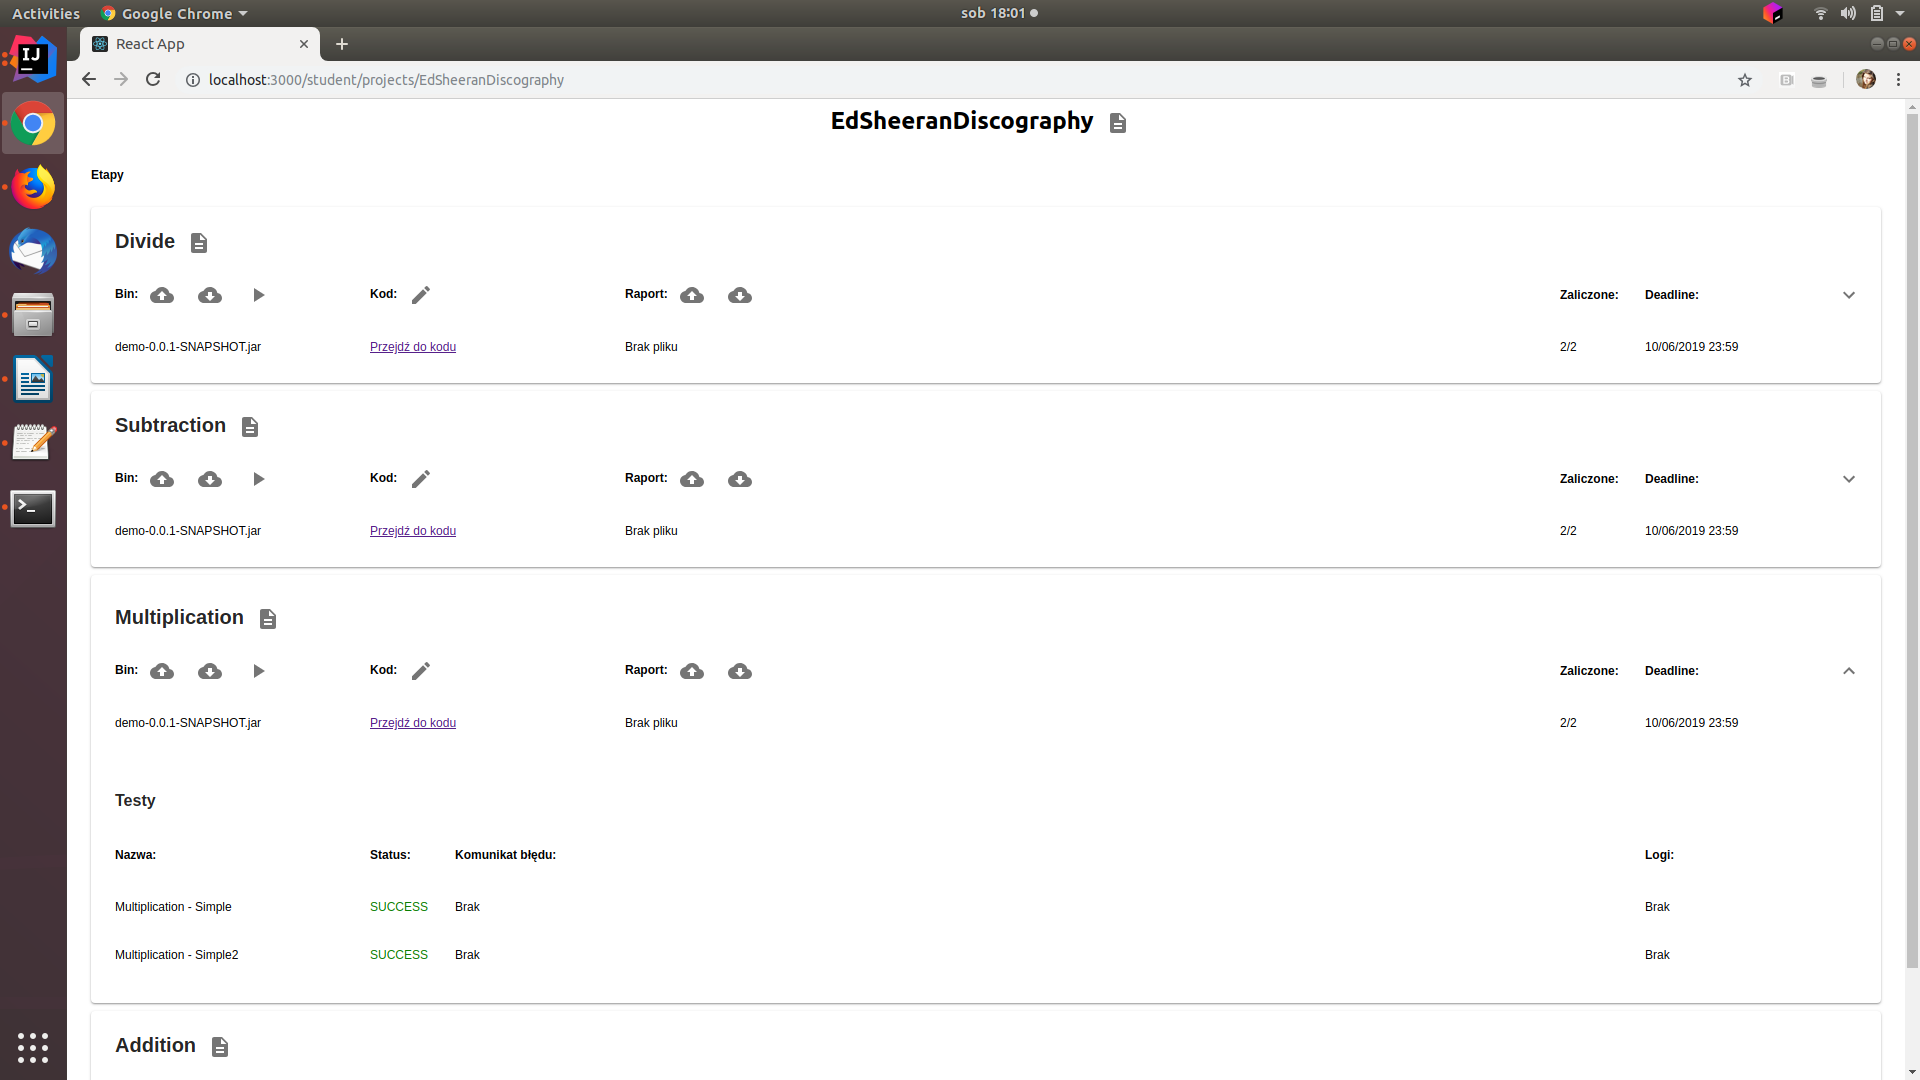
\includegraphics[width = 13cm]{chapter04/lecturer_interface_view.png}
    \caption{Interfejs prowadzącego - podgląd postępów studentów (źródło własne).}
    \label{fig:lecturer-interface-view}
\end{figure}

Prowadzący ma umożliwiony wgląd w:
\begin {itemize}
    \item Aktualną punktację projektu dla grupy.
    \item Liczbę prób podjętych przez daną grupę, dla każdego z etapów.
    \item Daty wykonania poszczególnych prób oraz ich statusy.
    \item Pełne komunikaty błędów i logi z ostatniej wykonanej przez studentów próby.
    \item Link do kodu źródłowego, który został użyty przez studentów do zbudowania programu.
    \item Sprawozdanie wykonane dla zadanego etapu.
\end {itemize}


\subsubsection{Pogląd postępów w ramach integracji}




\section{Interfejs studenta}

\subsubsection{Pogląd postępów w ramach etapu}

\subsubsection{Pogląd postępów w ramach integracji}

Na rysunku \ref{fig:student-interface} został przedstawiony interfejs studenta.
Umożliwia on dodawanie i edycję danych dla kolejnych etapów projektu oraz podgląd aktualnych postępów.
W ramach projektu student ma między innymi dostęp do dwóch plików: z opisem zadania oraz definicją środowiska Dockerowego.
Interfejs umożliwia też dostęp do opisów kolejnych etapów, terminów ich realizacji i punktacji.

Dla zadanego etapu student ma możliwość załączenia:
\begin {itemize}
    \item Pliku wykonywalnego z programem, który będzie testowany na platformie.
    \item Linku do kodu, z którego został zbudowany plik wykonywalny.
    \item Sprawozdania, sporządzonego w ramach etapu.
\end {itemize}

Po załączeniu programu student ma możliwość uruchomienia go na platformie.
Wynik działania programu jest przedstawiony studentowi w postaci listy rezultatów z wykonania poszczególnych przypadków testowych.
Poszczególny rekord zawiera informacje o:
\begin {itemize}
    \item Nazwie przypadku testowego, którego dotyczy wynik.
    \item Parametrach wejściowych, które zostały użyte przy uruchomieniu programu.
    \item Statusie wykonania przypadku testowego (sukces/porażka).
    \item Komunikatu błędu, w przypadku porażki.
    \item Pliku z logami z wykonania danego przypadku testowego.
\end{itemize}

W ramach podglądu postępów student ma dostęp do:
\begin {itemize}
    \item Wyników wszystkich dotychczasowych etapów.
    \item Informacji zbiorczej o liczbie zaliczonych etapów i aktualnej punktacji.
    \item Zbiorczej informacji o postępach innych grup.
    Informacja ta jest przedstawiono jako liczba grup, które zaliczyły wskazany etap w stosunku do wszystkich grup.
\end {itemize}

Student po zakończeniu odpowiedniej liczby etapów wchodzących w skład zdefiniowanego procesu integracji ma możliwość uruchomienia tego procesu.
Wynik działania procesu jest reprezentowany w taki sam sposób jak wynik uruchomienia poszczególnego etapu.